\documentclass[]{article}
\usepackage{lmodern}
\usepackage{amssymb,amsmath}
\usepackage{ifxetex,ifluatex}
\usepackage{fixltx2e} % provides \textsubscript
\ifnum 0\ifxetex 1\fi\ifluatex 1\fi=0 % if pdftex
  \usepackage[T1]{fontenc}
  \usepackage[utf8]{inputenc}
\else % if luatex or xelatex
  \ifxetex
    \usepackage{mathspec}
  \else
    \usepackage{fontspec}
  \fi
  \defaultfontfeatures{Ligatures=TeX,Scale=MatchLowercase}
\fi
% use upquote if available, for straight quotes in verbatim environments
\IfFileExists{upquote.sty}{\usepackage{upquote}}{}
% use microtype if available
\IfFileExists{microtype.sty}{%
\usepackage[]{microtype}
\UseMicrotypeSet[protrusion]{basicmath} % disable protrusion for tt fonts
}{}
\PassOptionsToPackage{hyphens}{url} % url is loaded by hyperref
\usepackage[unicode=true]{hyperref}
\hypersetup{
            pdfborder={0 0 0},
            breaklinks=true}
\urlstyle{same}  % don't use monospace font for urls
\usepackage{graphicx,grffile}
\makeatletter
\def\maxwidth{\ifdim\Gin@nat@width>\linewidth\linewidth\else\Gin@nat@width\fi}
\def\maxheight{\ifdim\Gin@nat@height>\textheight\textheight\else\Gin@nat@height\fi}
\makeatother
% Scale images if necessary, so that they will not overflow the page
% margins by default, and it is still possible to overwrite the defaults
% using explicit options in \includegraphics[width, height, ...]{}
\setkeys{Gin}{width=\maxwidth,height=\maxheight,keepaspectratio}
\IfFileExists{parskip.sty}{%
\usepackage{parskip}
}{% else
\setlength{\parindent}{0pt}
\setlength{\parskip}{6pt plus 2pt minus 1pt}
}
\setlength{\emergencystretch}{3em}  % prevent overfull lines
\providecommand{\tightlist}{%
  \setlength{\itemsep}{0pt}\setlength{\parskip}{0pt}}
\setcounter{secnumdepth}{0}
% Redefines (sub)paragraphs to behave more like sections
\ifx\paragraph\undefined\else
\let\oldparagraph\paragraph
\renewcommand{\paragraph}[1]{\oldparagraph{#1}\mbox{}}
\fi
\ifx\subparagraph\undefined\else
\let\oldsubparagraph\subparagraph
\renewcommand{\subparagraph}[1]{\oldsubparagraph{#1}\mbox{}}
\fi

% set default figure placement to htbp
\makeatletter
\def\fps@figure{htbp}
\makeatother


\date{}

\begin{document}

Работа 3.4.3

Точка Кюри

\begin{quote}
\textbf{Цель работы:} определение точки Кюри ферромагнетиков по
темпе­ратурным зависимостям магнитной проницаемости и сопротивления.

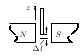
\includegraphics{./media/image1.png}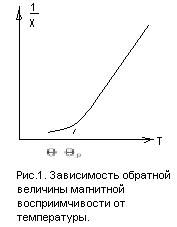
\includegraphics{./media/image2.png}\textbf{В
работе используются:} трансформатор, катушки, амперметры, вольтметры,
реостаты, трубчатая печь, цифровой вольтметр, термо­пары, образцы.
\end{quote}

В первой части работы исследуется изменение начальной магнитной
проницаемости ферромагнетика вблизи точки Кюри θ ( рис. 1), во второй
--- зависимость сопротивления образца от температуры (фазовый переход
П-го рода --- рис. 2).

Известно, что в ферромагнетике при определённой температуре, на­зываемой
\emph{точкой Кюри,} исчезает спонтанная намагниченность матери­ала. Это
сопровождается изменением ряда физических свойств ферро­магнетика:
теплоёмкости, теплопроводности, электропроводности, маг­нитной
восприимчивости и проницаемости; исчезает эффект магнитострикции и
анизотропия намагниченности. Поэтому, нагревая ферромагнитный образец и
наблюдая за изменением его физических свойств, можно определить точку
Кюри ферромагнетика.

А. Определение точки Кюри по изменению магнитной проницаемости

\textbf{Экспериментальная установка,} представленная на рис. 3, состоит
из намагничивающей катушки \emph{L,} питаемой переменным током, и
из­мерительной катушки \emph{L\textsubscript{1},} замкнутой через диод
\emph{D} на микроамперметр \emph{А\textsubscript{1}.}

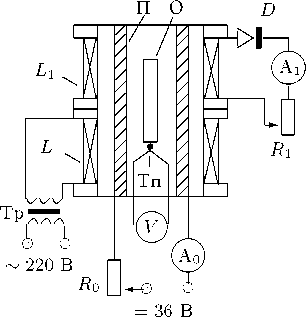
\includegraphics{./media/image3.png}

Рис. 3. Схема экспериментальной установки для исследования д(Т)

При прохождении переменного тока через катушку \emph{L} в ка­тушке
\emph{L\textsubscript{1}} возникает индукционный ток I\textsubscript{1}.
Величину тока можно регу­лировать реостатом \emph{R\textsubscript{1}.}

Внутри обеих катушек находится небольшая трубчатая печь П, в ко­торую
помещается образец О. Печь нагревается бифилярной обмоткой, подключённой
к источнику постоянного напряжения 36 В. Ток нагрева печи Iо можно
регулировать реостатом и контролировать ампермет­ром \emph{Ао.}

Нагрев катушек \emph{L} и \emph{L\textsubscript{1}} может изменить их
сопротивления и сказать­ся на показаниях микроамперметра. Для уменьшения
вредного нагрева в зазор между печкой и катушками вдувается воздух с
помощью вен­тилятора. Напряжение питания вентилятора --- 36 В.

Температура внутри печи измеряется с помощью термопары Тп, со­единённой
с милливольтметром \emph{V.} По показаниям милливольтметра можно с
помощью графика чувствительности термопары, приведённо­го на установке,
определить температуру спая термопары относительно комнатной, а затем,
зная комнатную температуру, найти температуру образца.

При неизменных прочих условиях ток индукции I\textsubscript{1} зависит
только от магнитной проницаемости образца, помещённого в печь, т. е.
I\textsubscript{1} = = f(μ). Это утверждение легко проверить, сняв
зависимость тока I\textsubscript{1} от температуры печи, когда в ней нет
образца, и с ферромагнитным образцом. В первом случае ток практически не
зависит от температу­ры печи, а во втором --- изменение тока будет
значительным вблизи точки Кюри (рис. 1). При температуре выше точки Кюри
показания микроамперметра будут такими же, как и в отсутствие образца.

Точка Кюри соответствует середине участка с максимальным накло­ном
касательной к кривой; рабочий диапазон Δ\emph{Т} должен быть несколь­ко
шире.

ЗАДАНИЕ

В этом упражнении предлагается снять зависимость тока индукции от
температуры и рассчитать точку Кюри для двух образцов. В работе
исследуются стержни из ферромагнитных материалов (никель и пермендюр) и
феррита.

\begin{enumerate}
\def\labelenumi{\arabic{enumi}.}
\item
  Перед началом работы с помощью графика чувствительности термо­пары
  рассчитайте предельно допустимую разность потенциалов, если известно,
  что температура образца не должна превышать 400 °С.
\item
  Поместив ферромагнитный стержень в катушку, включите трансфор­матор Тр
  в сеть на 220 В. Образец следует опустить до упора, под которым
  расположена термопара.
\item
  С помощью потенциометра \emph{R\textsubscript{1}} установите в цепи
  катушки L\textsubscript{1} ток I1, вызывающий отклонение стрелки
  микроамперметра примерно на 3/4 шкалы.
\item
  Установите реостат Rо в среднее положение и подключите печь к
  ис­точнику 36 В. Тумблером, расположенным под катушками, включите
  вентилятор.
\item
  Подберите режим, удобный для определения точки Кюри: чтобы быстрее
  дойти от комнатной температуры до начала рабочего участ­ка Δ\emph{Т}
  (рис. 1), установите максимальный ток нагрева печи (Iо
  \textasciitilde{} 5 А) с помощью реостата Rо. Заметив начало спада
  тока индукции, умень­шите ток нагрева вдвое. Оцените границы рабочего
  диапазона термопа­ры Δ\emph{U} (\textasciitilde{}ΔТ) и интервал
  резкого изменения тока . Максимальный ток A1 должен быть близок к
  концу шкалы.
\end{enumerate}

Не перегревайте катушку! (см. п. 1).

Подберите ток нагрева Iо так, чтобы время одной серии (нагрев или
охлаждение внутри рабочего диапазона Δ\emph{U)} составляло 2-3 мин. В
течение одной серии не следует менять чувствительность микроам­перметра
(I1) и ток нагрева печи (Iо), т. к. это влияет на величину тока индукции
I\textsubscript{1}.

Проведите предварительные измерения: при фиксированном токе нагрева Iо
регистрируйте I\textsubscript{1} \textbf{и U} (дел). Полезно отметить
время начала и окончания записи, чтобы оценить продолжительность одной
серии.

\begin{enumerate}
\def\labelenumi{\arabic{enumi}.}
\item
  Выбрав режим работы, снимите зависимость тока индукции
  I\textsubscript{1} от термо-ЭДС \emph{U} при постоянном токе Iо; в
  области резкого изменения
\end{enumerate}

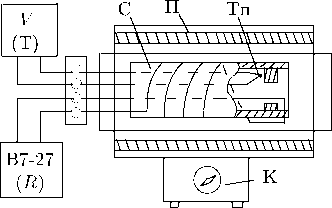
\includegraphics{./media/image4.png}

Рис. 4. Схема экспериментальной установки для исследования \emph{R(T)}

тока I\textsubscript{1} точки должны лежать почаще. Проведите измерения
при нагревании и охлаждении образца.

\begin{enumerate}
\def\labelenumi{\arabic{enumi}.}
\item
  Повторите п. 2-6 для второго образца.
\item
  Охладив катушку, отключите печь и ток намагничивания.
\end{enumerate}

Обработка результатов

\begin{enumerate}
\def\labelenumi{\arabic{enumi}.}
\item
  Постройте графики I\textsubscript{1} \emph{=} f(T) (дел){]}, не
  пересчитывая каждую точ­ку в Δ\emph{Т} °С. Определите точку Кюри как
  температуру средней точки участка кривой с максимальным наклоном
  касательной (в единицах \emph{U} дел).
\end{enumerate}

Для выбранной точки пересчитайте \emph{U} (дел) сначала в милливольты
(150 дел --- 45 мВ), а затем по графику чувствительности термопары --- в
Δ\emph{Т} °С. Зная комнатную температуру, определите температуру Кю­ри
θ.

\begin{enumerate}
\def\labelenumi{\arabic{enumi}.}
\item
  Оцените погрешность и сравните результат с табличным.
\end{enumerate}

Б. Определение точки Кюри по изменению сопротивления

\textbf{Экспериментальная установка} для исследования зависимости
омического сопротивления ферромагнетика от температуры представ­лена на
рис. 4. Никелевая спираль С, намотанная на фарфоровую труб­ку, заключена
в керамическую трубку и помещена в трубчатую печь П. Нагрев печи
регулируется переключателем К. Температура фарфоро­вой трубки (спирали)
контролируется термопарой Тп, подключённой к милливольтметру \emph{V,}
прокалиброванному в градусах. Сопротивление спирали измеряется цифровым
вольтметром В7-27.

ЗАДАНИЕ

В этом упражнении предлагается снять зависимость сопротивления никелевой
спирали от температуры и определить точку Кюри.

\begin{enumerate}
\def\labelenumi{\arabic{enumi}.}
\item
  Включите в сеть цифровой вольтметр. Измерьте сопротивление ни­келевой
  спирали при комнатной температуре \emph{(R} \textasciitilde{} 10 Ом).
\item
  Включите печь в сеть на 220 В и поставьте переключатель К в среднее
  положение.
\item
  Измеряйте сопротивление \emph{R} и температуру спирали \emph{Т} через
  каж­дые 20 градусов, не останавливая нагрева. При температуре образца
  \textgreater{} 200 °С мощность нагрева следует увеличить.
\end{enumerate}

Дойдя до предельной температуры \emph{(Т}\textsubscript{тах} = 450 °С),
отключите на­грев и проведите измерения при охлаждении образца до 100
°С.

Обработка результатов

\begin{enumerate}
\def\labelenumi{\arabic{enumi}.}
\item
  Постройте графики \emph{R = f(U\textsubscript{дел}).} По изменению
  температурного коэф­фициента сопротивления (пересечению касательных к
  прямолинейным участкам графика \emph{R = f(T))} найдите точку Кюри
  (рис. 2).
\item
  Градуировка милливольтметра соответствует термопаре железо-константан.
  Если в установке используется медь-константан, сделайте пе­ресчёт
  точки Кюри θ, используя графики чувствительности обеих тер­мопар (не
  забудьте учесть комнатную температуру --- обычно ≈20 °С).
\item
  Оцените погрешности и сравните результат с табличным.
\end{enumerate}

Контрольные вопросы

\begin{enumerate}
\def\labelenumi{\arabic{enumi}.}
\item
  Чем отличаются атомы пара- и диамагнетиков по магнитным
  характери­стикам в отсутствие магнитного поля?
\item
  Как изменяются характеристики вещества при фазовых переходах первого и
  второго рода?
\end{enumerate}

3. Какие два конкурирующих взаимодействия между атомами характерны для
ферромагнитного вещества?

4. На одном графике качественно изобразите начальные кривые
намагничи­вания \emph{В(Н)} для ферромагнетика при трёх температурах:
комнатной, более высокой и температуре выше точки Кюри. Укажите на оси
\emph{Н,} где лежит область, соответствующая условиям настоящей работы.

СПИСОК ЛИТЕРАТУРЫ

\begin{enumerate}
\def\labelenumi{\arabic{enumi}.}
\item
  \emph{Сивухин Д.В.} Общий курс физики. Т. III. Электричество. --- М.:
  Наука, 1983. §§ 74, 79.
\item
  \emph{Калашников С.Г.} Электричество. --- М.: Наука, 1977. Гл. XI, §§
  110, 111, 119.
\end{enumerate}

\end{document}
